\chapter{Protecting Unsecure Web Application}
\label{Protecting Unsecure Web Application}
\section{Introduction}
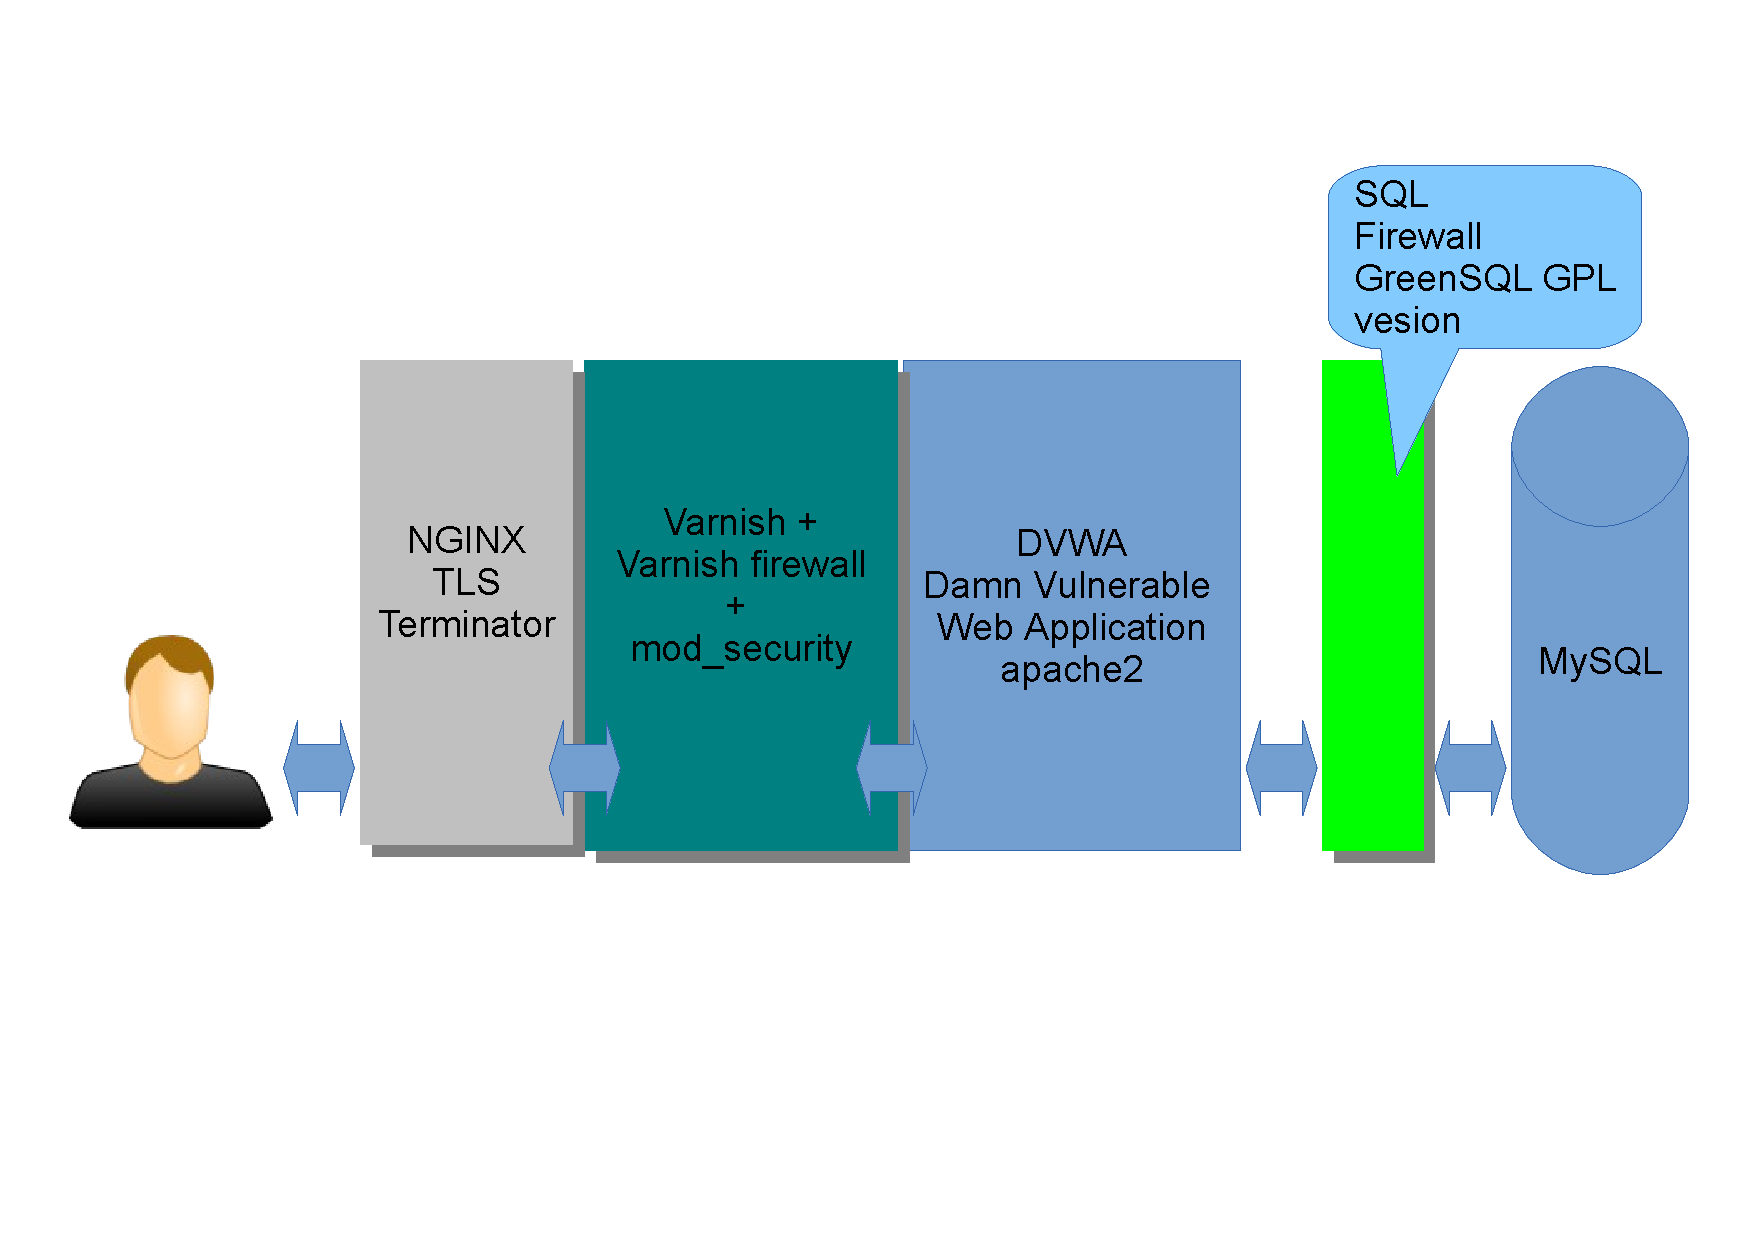
\includegraphics[width=\textwidth]{web_security_lab_goal.pdf}
\section{Pre-Requirements} 
\section{Scope}
\section{Learning Outcomes} 
\section{Setting up the Virtual Environment}
\section{Installation of Damn Vulnerable Web Application}
\subsection{Introduction to DVWA}

Ensure that you have administrator rights
\mint[frame=lines, framesep=1mm]{bash}|sudo -i|
Ensure that unzip package is installed
\begin{minted}[frame=lines,framesep=2mm]{bash}
type unzip || apt-get install unzip
\end{minted}
Dowload DVWA using web get utility wget
\mint[frame=lines, framesep=1mm]{bash}|wget http://dvwa.googlecode.com/files/DVWA-1.0.7.zip|

\begin{minted}[frame=lines,framesep=2mm]{bash}
unzip DVWA-1.0.7.zip
mv dvwa /var/www
http://192.168.56.200/dvwa/
nano /var/www/dvwa/config/config.inc.php

$_DVWA[ 'db_user' ] = 'root';
$_DVWA[ 'db_password' ] = 'student';
$_DVWA[ 'db_database' ] = 'dvwa';
\end{minted}
%$
For save use  CTRL + X

Username : admin
Password : password
Change DVWA Security level to low (for beginners)


